

% Gradient Info

\tikzset {_evaqk6wzt/.code = {\pgfsetadditionalshadetransform{ \pgftransformshift{\pgfpoint{0 bp } { 0 bp }  }  \pgftransformscale{1 }  }}}
\pgfdeclareradialshading{_1n0vthefz}{\pgfpoint{0bp}{0bp}}{rgb(0bp)=(0.95,0.98,1);
	rgb(0bp)=(0.95,0.98,1);
	rgb(25bp)=(0.84,0.94,0.99);
	rgb(400bp)=(0.84,0.94,0.99)}
\tikzset{every picture/.style={line width=0.75pt}} %set default line width to 0.75pt        

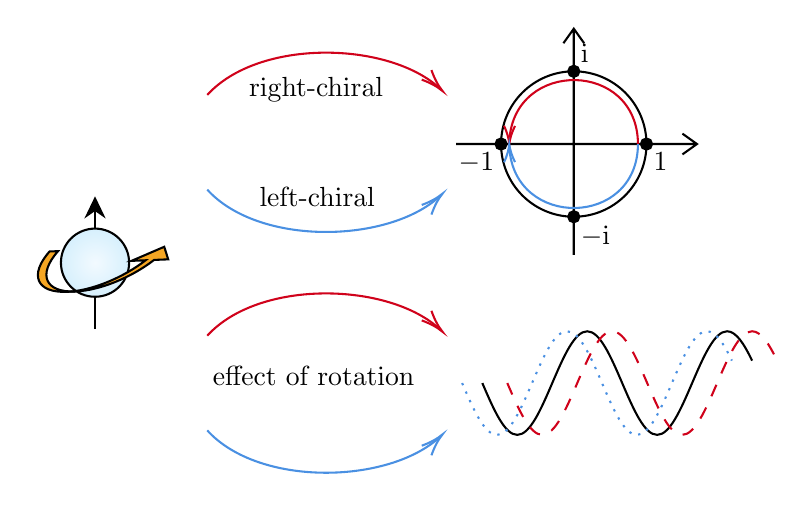
\begin{tikzpicture}[x=0.75pt,y=0.75pt,yscale=-1,xscale=1]
	%uncomment if require: \path (0,225); %set diagram left start at 0, and has height of 225
	
	%Straight Lines [id:da7572743314001158] 
	\draw [fill={rgb, 255:red, 144; green, 19; blue, 254 }  ,fill opacity=1 ]   (177.75,147.25) -- (177.75,86.27) ;
	\draw [shift={(177.75,83.27)}, rotate = 450] [fill={rgb, 255:red, 0; green, 0; blue, 0 }  ][line width=0.08]  [draw opacity=0] (10.72,-5.15) -- (0,0) -- (10.72,5.15) -- (7.12,0) -- cycle    ;
	%Shape: Ellipse [id:dp2822082850827441] 
	\path  [shading=_1n0vthefz,_evaqk6wzt] (161.32,115.26) .. controls (161.32,106.19) and (168.67,98.83) .. (177.75,98.83) .. controls (186.82,98.83) and (194.17,106.19) .. (194.17,115.26) .. controls (194.17,124.33) and (186.82,131.68) .. (177.75,131.68) .. controls (168.67,131.68) and (161.32,124.33) .. (161.32,115.26) -- cycle ; % for fading 
	\draw  [color={rgb, 255:red, 0; green, 0; blue, 0 }  ,draw opacity=1 ] (161.32,115.26) .. controls (161.32,106.19) and (168.67,98.83) .. (177.75,98.83) .. controls (186.82,98.83) and (194.17,106.19) .. (194.17,115.26) .. controls (194.17,124.33) and (186.82,131.68) .. (177.75,131.68) .. controls (168.67,131.68) and (161.32,124.33) .. (161.32,115.26) -- cycle ; % for border 
	
	%Curve Left Arrow [id:dp26723489796076993] 
	\draw  [fill={rgb, 255:red, 245; green, 166; blue, 35 }  ,fill opacity=1 ] (164.26,129.29) .. controls (149.57,129.89) and (145.8,121.19) .. (155.84,109.86) -- (159.94,109.7) .. controls (149.9,121.02) and (153.66,129.72) .. (168.36,129.12) ;\draw  [fill={rgb, 255:red, 245; green, 166; blue, 35 }  ,fill opacity=1 ] (168.36,129.12) .. controls (180.17,128.64) and (195.45,122.29) .. (206.2,113.93) -- (213,113.65) -- (211.1,107.6) -- (195.31,114.38) -- (202.11,114.1) .. controls (191.35,122.46) and (176.08,128.8) .. (164.26,129.29)(168.36,129.12) -- (164.26,129.29) ;
	
	%Shape: Axis 2D [id:dp22064170995903698] 
	\draw  (351.78,58.09) -- (467.76,58.09)(408.41,2.53) -- (408.41,111.54) (460.76,53.09) -- (467.76,58.09) -- (460.76,63.09) (403.41,9.53) -- (408.41,2.53) -- (413.41,9.53)  ;
	%Shape: Ellipse [id:dp8524966468602786] 
	\draw   (373.38,58.09) .. controls (373.38,38.74) and (389.06,23.06) .. (408.41,23.06) .. controls (427.75,23.06) and (443.43,38.74) .. (443.43,58.09) .. controls (443.43,77.44) and (427.75,93.12) .. (408.41,93.12) .. controls (389.06,93.12) and (373.38,77.44) .. (373.38,58.09) -- cycle ;
	%Straight Lines [id:da49553294322242825] 
	\draw    (443.43,58.09) ;
	\draw [shift={(443.43,58.09)}, rotate = 0] [color={rgb, 255:red, 0; green, 0; blue, 0 }  ][fill={rgb, 255:red, 0; green, 0; blue, 0 }  ][line width=0.75]      (0, 0) circle [x radius= 2.68, y radius= 2.68]   ;
	%Straight Lines [id:da5984806110215237] 
	\draw    (408.41,23.06) ;
	\draw [shift={(408.41,23.06)}, rotate = 0] [color={rgb, 255:red, 0; green, 0; blue, 0 }  ][fill={rgb, 255:red, 0; green, 0; blue, 0 }  ][line width=0.75]      (0, 0) circle [x radius= 2.68, y radius= 2.68]   ;
	%Straight Lines [id:da8369323246524298] 
	\draw    (408.41,93.12) ;
	\draw [shift={(408.41,93.12)}, rotate = 0] [color={rgb, 255:red, 0; green, 0; blue, 0 }  ][fill={rgb, 255:red, 0; green, 0; blue, 0 }  ][line width=0.75]      (0, 0) circle [x radius= 2.68, y radius= 2.68]   ;
	%Straight Lines [id:da6270329877482388] 
	\draw    (373.38,58.09) ;
	\draw [shift={(373.38,58.09)}, rotate = 0] [color={rgb, 255:red, 0; green, 0; blue, 0 }  ][fill={rgb, 255:red, 0; green, 0; blue, 0 }  ][line width=0.75]      (0, 0) circle [x radius= 2.68, y radius= 2.68]   ;
	%Curve Lines [id:da23824647545105204] 
	\draw [color={rgb, 255:red, 208; green, 2; blue, 27 }  ,draw opacity=1 ]   (439.34,58.09) .. controls (439.11,17.61) and (379.76,17.01) .. (377.39,56.27) ;
	\draw [shift={(377.33,58.09)}, rotate = 270.85] [color={rgb, 255:red, 208; green, 2; blue, 27 }  ,draw opacity=1 ][line width=0.75]    (8.74,-2.63) .. controls (5.56,-1.12) and (2.65,-0.24) .. (0,0) .. controls (2.65,0.24) and (5.56,1.12) .. (8.74,2.63)   ;
	%Curve Lines [id:da6462902096310119] 
	\draw [color={rgb, 255:red, 74; green, 144; blue, 226 }  ,draw opacity=1 ]   (439.34,58.09) .. controls (439.11,98.57) and (379.76,99.17) .. (377.39,59.91) ;
	\draw [shift={(377.33,58.09)}, rotate = 449.15] [color={rgb, 255:red, 74; green, 144; blue, 226 }  ,draw opacity=1 ][line width=0.75]    (8.74,-2.63) .. controls (5.56,-1.12) and (2.65,-0.24) .. (0,0) .. controls (2.65,0.24) and (5.56,1.12) .. (8.74,2.63)   ;
	
	%Curve Lines [id:da2522351838052146] 
	\draw [color={rgb, 255:red, 208; green, 2; blue, 27 }  ,draw opacity=1 ]   (231.82,34.45) .. controls (256.8,6.96) and (319.63,8.57) .. (344.09,31.48) ;
	\draw [shift={(345.18,32.54)}, rotate = 225.34] [color={rgb, 255:red, 208; green, 2; blue, 27 }  ,draw opacity=1 ][line width=0.75]    (10.93,-3.29) .. controls (6.95,-1.4) and (3.31,-0.3) .. (0,0) .. controls (3.31,0.3) and (6.95,1.4) .. (10.93,3.29)   ;
	%Curve Lines [id:da02423372186453876] 
	\draw [color={rgb, 255:red, 74; green, 144; blue, 226 }  ,draw opacity=1 ]   (231.82,80.06) .. controls (256.8,107.56) and (319.63,105.95) .. (344.09,83.04) ;
	\draw [shift={(345.18,81.98)}, rotate = 494.66] [color={rgb, 255:red, 74; green, 144; blue, 226 }  ,draw opacity=1 ][line width=0.75]    (10.93,-3.29) .. controls (6.95,-1.4) and (3.31,-0.3) .. (0,0) .. controls (3.31,0.3) and (6.95,1.4) .. (10.93,3.29)   ;
	
	
	%Curve Lines [id:da40466147892473336] 
	\draw [color={rgb, 255:red, 208; green, 2; blue, 27 }  ,draw opacity=1 ]   (231.82,150.45) .. controls (256.8,122.96) and (319.63,124.57) .. (344.09,147.48) ;
	\draw [shift={(345.18,148.54)}, rotate = 225.34] [color={rgb, 255:red, 208; green, 2; blue, 27 }  ,draw opacity=1 ][line width=0.75]    (10.93,-3.29) .. controls (6.95,-1.4) and (3.31,-0.3) .. (0,0) .. controls (3.31,0.3) and (6.95,1.4) .. (10.93,3.29)   ;
	%Curve Lines [id:da11726096837131395] 
	\draw [color={rgb, 255:red, 74; green, 144; blue, 226 }  ,draw opacity=1 ]   (231.82,196.06) .. controls (256.8,223.56) and (319.63,221.95) .. (344.09,199.04) ;
	\draw [shift={(345.18,197.98)}, rotate = 494.66] [color={rgb, 255:red, 74; green, 144; blue, 226 }  ,draw opacity=1 ][line width=0.75]    (10.93,-3.29) .. controls (6.95,-1.4) and (3.31,-0.3) .. (0,0) .. controls (3.31,0.3) and (6.95,1.4) .. (10.93,3.29)   ;
	
	%Shape: Wave [id:dp9433948168752311] 
	\draw   (364.35,173.26) .. controls (369.84,186.04) and (375.1,198.22) .. (381.19,198.22) .. controls (387.29,198.22) and (392.55,186.04) .. (398.04,173.26) .. controls (403.53,160.47) and (408.79,148.3) .. (414.89,148.3) .. controls (420.99,148.3) and (426.24,160.47) .. (431.74,173.26) .. controls (437.23,186.04) and (442.49,198.22) .. (448.58,198.22) .. controls (454.68,198.22) and (459.94,186.04) .. (465.43,173.26) .. controls (470.93,160.47) and (476.18,148.3) .. (482.28,148.3) .. controls (486.59,148.3) and (490.47,154.38) .. (494.32,162.45) ;
	%Shape: Wave [id:dp5227264393253617] 
	\draw  [color={rgb, 255:red, 74; green, 144; blue, 226 }  ,draw opacity=1 ][dash pattern={on 0.84pt off 2.51pt}] (354.62,173.26) .. controls (360.11,186.04) and (365.37,198.22) .. (371.46,198.22) .. controls (377.56,198.22) and (382.82,186.04) .. (388.31,173.26) .. controls (393.81,160.47) and (399.06,148.3) .. (405.16,148.3) .. controls (411.26,148.3) and (416.51,160.47) .. (422.01,173.26) .. controls (427.5,186.04) and (432.76,198.22) .. (438.86,198.22) .. controls (444.95,198.22) and (450.21,186.04) .. (455.7,173.26) .. controls (461.2,160.47) and (466.45,148.3) .. (472.55,148.3) .. controls (476.86,148.3) and (480.75,154.38) .. (484.59,162.45) ;
	%Shape: Wave [id:dp18938055828073508] 
	\draw  [color={rgb, 255:red, 208; green, 2; blue, 27 }  ,draw opacity=1 ][dash pattern={on 4.5pt off 4.5pt}] (376.39,173.26) .. controls (381.88,186.04) and (387.14,198.22) .. (393.24,198.22) .. controls (399.33,198.22) and (404.59,186.04) .. (410.08,173.26) .. controls (415.58,160.47) and (420.84,148.3) .. (426.93,148.3) .. controls (433.03,148.3) and (438.29,160.47) .. (443.78,173.26) .. controls (449.27,186.04) and (454.53,198.22) .. (460.63,198.22) .. controls (466.72,198.22) and (471.98,186.04) .. (477.48,173.26) .. controls (482.97,160.47) and (488.23,148.3) .. (494.32,148.3) .. controls (498.63,148.3) and (502.52,154.38) .. (506.37,162.45) ;
	
	
	
	% Text Node
	\draw (233,163.45) node [anchor=north west][inner sep=0.75pt]   [align=left] {effect of rotation};
	% Text Node
	\draw (250.5,24.45) node [anchor=north west][inner sep=0.75pt]   [align=left] {right-chiral};
	% Text Node
	\draw (255.5,77.45) node [anchor=north west][inner sep=0.75pt]   [align=left] {left-chiral};
	% Text Node
	\draw (445.34,60.96) node [anchor=north west][inner sep=0.75pt]    {$1$};
	% Text Node
	\draw (371.52,60.96) node [anchor=north east] [inner sep=0.75pt]    {$-1$};
	% Text Node
	\draw (410.32,20.19) node [anchor=south west] [inner sep=0.75pt]    {$\mathrm{i}$};
	% Text Node
	\draw (410.28,95.99) node [anchor=north west][inner sep=0.75pt]    {$-\mathrm{i}$};
	
	
\end{tikzpicture}